%!TEX root = main.tex
\section{Recurrent Neural Network: Prediction} \label{sec:rnn_pred}

In addition to classification, we also investigated applying LSTMs to the task of pedestrian motion prediction.
That is, rather than a binary label, we try to predict \textit{where} the pedestrian will walk next.
This is much more challenging, but also would be more insightful to an end-user in vehicle applications.

\subsection{Introduction}
Existing research has been conducted in predicting trajectories in a 2D space. 
One relevant work used LSTMs to generate human handwriting from the IAM online handwriting database~\cite{DBLP:journals/corr/Graves13}.

LSTMs can be used to predict sequences, by feeding themselves their output as an input.
To switch from binary classification to trajectory predicting LSTM, we change the network architecture from many-to-one to many-to-many.
The output $y_t \Re^{Tx2}$ is computed from every time step as given in ~\cref{eq:eq:bin_class_out}.

Many works can be found for the task of text prediction (e.g. \cite{ICML2011Sutskever_524}).
However, our application domain is real-valued, as opposed to the discrete-valued domain of word prediction.

The literature proposes several transformations, which could be applied to the output $y_t$.
For example, (Graves) uses mixture density networks (MDNs) and calculates $x_{t+1}$ by the conditional probability $P(x_{t+1}|y_t, )$ and uses a Gaussian mixture prior on the probability distribution.
The loss is the negative-log likelihood of the conditional probability, and SGD is applied to update the weights along with the parameters of the distribution: mean $\mu_m$, standard deviation $\sigma_m$, correlation $\rho_m$, mixture weights $\pi_m$ for $M$ mixture components.
However, the proposed transition function is quite complicated and leads to longer training time, which is not promising. 

Additionally, (graves) used the relative position between timesteps $\delta x = x_{t+1} - x_t$ as input vector.
In our case, we cannot use the relative position, because we would lose the information of proximity to the car.
In other words, we would ignore that a pedestrian might avoid an approaching car.
For the MDN approach, our means $\mu_m$ would be further spread among the full absolute position space, which would presumably require even longer training time than the earlier approach.
Therefore, we have decided to linearly compute the output, as stated in ~\cref{eq:bin_class_out}. 

As we cannot use the loss function proposed by (graves), our chosen loss function is the mean squared error of each predicted output and next ground truth input, over the whole time sequence.
We have used the $L_2$ norm instead of the $L_1$ norm to be more robust against outliers.

\begin{equation}
Loss_{pred}(x_t) = \frac{1}{T} \sum_{t=0}^{T}(y_t - x_{t+1})^2
\label{eq:loss_pred} 
\end{equation}
%TODO write about last point.

% random batch
The loss function is computed for every batch and we update the parameters in the activation cells via SGD.
We randomly draw batches from our training dataset for each SGD parameter update.
Therefore, we break apart the dependency of previously concatenated trajectories, that we have split apart into snippets.
This is necessary, as a test trajectory will be independent of the training trajectories.

% prediction, parameter-sharing
For prediction, the parameter-sharing property of RNNs and LSTMs is essential.
The activation units' parameters have been trained to predict the next state based on the current state.
Therefore, for prediction, where the ground truth input vector is unkown, the LSTM can use the output $y_{t-1}$ as input for $x_t$.
This gives us the predicted pedestrian position $y_t$.

\subsection{Generated Data}
As seen in the previous sections, the given pedestrian trajectories are highly complex nonlinear functions.
To validate our LSTM prediction model, we have instead tested on simpler functions. Therefore, we have chosen to generate linear and sinusodial shaped trajectories, displayed in ~\cref{fig:lin_sin_traj}.

\begin{figure}
	\centering
	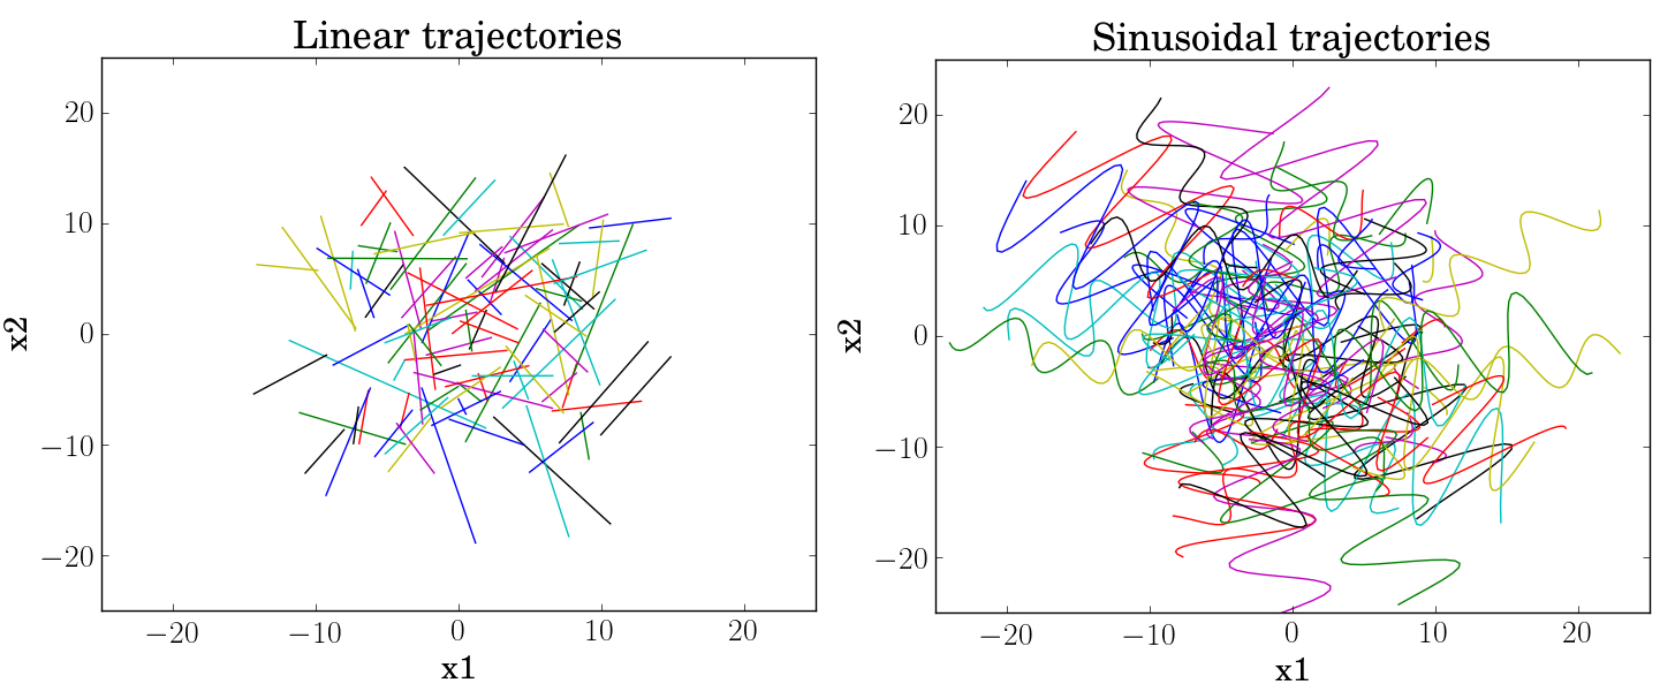
\includegraphics [trim=0 0 0 0, clip, angle=0, width=1.0\columnwidth,
	keepaspectratio]{figures/lin_sin_traj}
	\caption{Randomly generated trajectory data in linear (left) shape and sinusodial shape (right). The trajectories have been generated by sampling the start point, range, scale, translation and rotation at random.} 
	\label{fig:lin_sin_traj} 
\end{figure}
%TODO fit linear data
For our hyperparameter tuning, we considered the batch size $b$, number of training samples $N$, snippet length $T$, learning rate $lr$, maximum epochs $e_{max}$ and number of hidden units $n_h$. 
As the possible combinations rise exponentially with the number of parameters and our computational resources are very limited, we have evaluated most of the parameters, while holding the other parameters constant.
Optimal tuning would run a search over all combinations, which would result in better performance.

In the search over the number of hidden units we made the following observations.
As seen in ~\cref{fig:rnn_hidden}, the number of hidden units $n_h = 1$ is insufficient to represent the complexity of sinusodial curves.
We can also see, that the complexity of $n_h=4$ is sufficient to approximately fit the sinusodial shape, and $n_h=32$ is sufficient to fit the data very well (upon visual inspection).


\begin{figure}
	\centering
	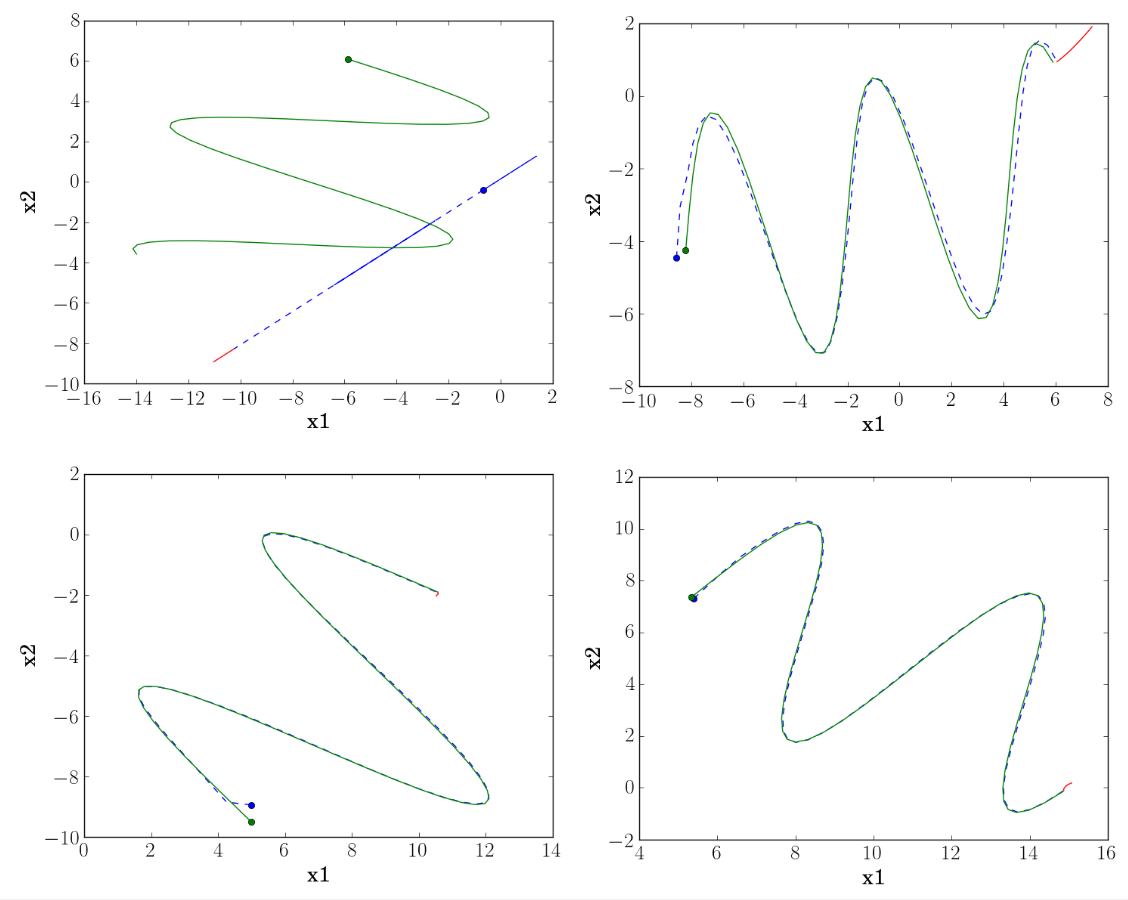
\includegraphics [trim=0 0 0 0, clip, angle=0, width=1.0\columnwidth,
	keepaspectratio]{figures/rnn_hidden}
	\caption{Search over the number of hidden units: $n_h=1$(top-left), $n_h=4$(top-right), $n_h=32$(bottom-left), $n_h=128$(bottom-right). The plot displays the input trajectory (green) $x_t$ with total trajectory snippet length $T=50$ an its starting point (green-dot). The LSTM predicts the next pedestrian position $y_t$ (blue-dotted) with its starting point (blue-dot), based on the past sequence $x_{0:t}$ and the learned parameters. After the input trajectory (green) is finished, the LSTM tries to predict the future trajectory (red) for $T_p=10$ timesteps. All trajectories are test trajectories and have not been included in the training set.}
	\label{fig:rnn_hidden}
\end{figure}

In ~\cref{tab:rnn_hidden} we see that increasing the number of hidden nodes $n_h$ shrinks the loss.
The training time exponentially increases with the number of hidden units, which makes us prefer a lower number of hidden units.
A high number of hidden units suggests an overfitting on the training data.
However, we can see that our independently generated test data shows similar error as the training set.
The more complex the model, the fewer epochs it took to reach an acceptable loss value.
Moving forward, we refer to the models with the hyperparameters from ~\cref{tab:rnn_hidden} as 1-, 4-, 32- and 128-unit model.

We used early stopping (based on a validation dataset) to prevent overfitting.
The training was stopped when the difference in average batch loss between two consecutive epochs $\delta L_b < 0.001$.


\begin{table}[]
\centering
\begin{tabular}{ c| c| c| c| c}
& $n_h=1$ & $n_h=4$ &$n_h=32$ & $n_h=128$\\
\hline
$L_e=0$ & 58.5 & 49.7  & \textbf{6.22} & 2.62      \\
$L_e=1$ & 54.2 & 36.0  & \textbf{0.50} & 0.12      \\
$L_e=2$ & 51.1 & 24.4  & \textbf{0.23} & 0.05      \\
$L_e=3$ & 49.2 & 17.8  & \textbf{0.14} & 0.03      \\
\hline
$e_c$ 			& 25 	& 85 	& 35	& 10 		\\
$L_{e_c}$		&  0.30	& 0.03	& 0.0058& 0.004 	\\
$L_{test, e_c}$	& 0.34	& 0.04	&0.003	& 0.003 	\\     
\end{tabular}
\caption{Search over the number of hidden units $n_h$. The average batch loss ($b=100$) over epochs $e$ and test loss is displayed. Number of training samples $N = 5000$ with snippet length $T=50$ and learning rate $lr=0.01$.}
\label{tab:rnn_hidden}
\end{table}

Include oscillating plot for convergence property.
~\cref{fig:rnn_hidden} also illustrates how LSTM starts by guessing $y_0$ purely based on the input $x_0$. 

% minimum snippet length.
Our tuning showed, that the model needs a minimum snippet length to be able to estimate the curve.
For very low snippet length ($T<10$) our loss increased ($Loss_b=0.02$ for model $n_h=4$ from ~\cref{tab:rnn_hidden}).
An increase in the snippet length over the threshold snippet length $T=50$ was not observed.
Therefore, we have set the default snippet length to $T=50$.

% learning rate, TODO include plot of oscillating learning rate.
The learning rate $lr$ influences the rate of convergence.
The higher, the faster the model should converge.
However, too high values of the learning rate can cause an oscillation over the minimum or divergence.
In our case, all learning rates in the interval $[0.1, 0.01, 0.001, 0.0001]$ have led to a reasonably low loss.
$Lr=0.1$ made the loss oscillate in the interval $[0.01, 0.07]$ for our 32-unit model.
A learning rate of $lr=0.01$ for the 32-unit model showed the best tradeoff in terms of minimal loss, while maintaining fast training.

% batch size 
Our choice of batch size $b$ impacted the speed of converges, because tf is possible to execute efficient matrix operations, but did not impact the achievable loss given a fixed model and infinite possible epochs.
Given a dataset of size $N=5000$, we have chosen the batch size to be $b=100$.

%Prediction accuracy.
The LSTM has been designed to predict an unseen pedestrian trajectory for a given number of time steps.
Previous work has shown that an LSTM is generally possible to predict a sinusoidial curve into the future~\cite{sunsided}.
However, they use $x_1$ as the input and predict the $x_2$ value.
This is not directly possible in our case, as we have to predict in a local frame with respect to the car.
Therefore, we predict both variables at the same time $x = (x_1, x_2)$, making the learning task more complex.
Additionally, previous work uses more complex models ($n_h=150$) with more training data ($N>500000$) and lower learning rate ($lr<0.0005$).
The number of epochs is not stated.
An iteration over other hyperparameter choices with these values is not feasible for the scope of this project.
However, the work suggests that further optimization of the hyperparameters would make it possible to predict trajectories.
The red line in ~\cref{fig:rnn_hidden} displays the predictions by our model. 

We conclude that our model is able to predict one step into the future accurately, given our achieved average batch loss $L_b<0.006$.
However, an accurate prediction over many timesteps requires more computational power for hyperparameter tuning. 

\subsection{Real pedestrian data}

We have shown that our LSTM is able continuously predict the next timestep in a domain of translated, rotated, scaled and stretched sinusoidial trajectories. The real pedestrian trajectories are highly nonlinear. LSTMs, in fact neural networks in general, show the capability of fitting a function onto the highly nonlinear data. In ~\cref{fig:ped_data} we can see the trajectories being predicted by our LSTM model.

%TODO add dataset length
We have trained, validated and tested on distinct datasets. All hyperparameters have been chosen based on the results of the sinusodial trajectories and re-validated for the new domain. ~\cref{fig:rnn_real_ped} and ~\cref{tab:rnn_real_ped} shows the performance of our LSTM on real pedestrian data. The learning rate is $lr=0.01$, batch-size $b=100$. 

Additionally, pedestrians behave irrational, do not follow predestined rules and different pedestrians behave differently. 

\begin{figure}
	\centering
	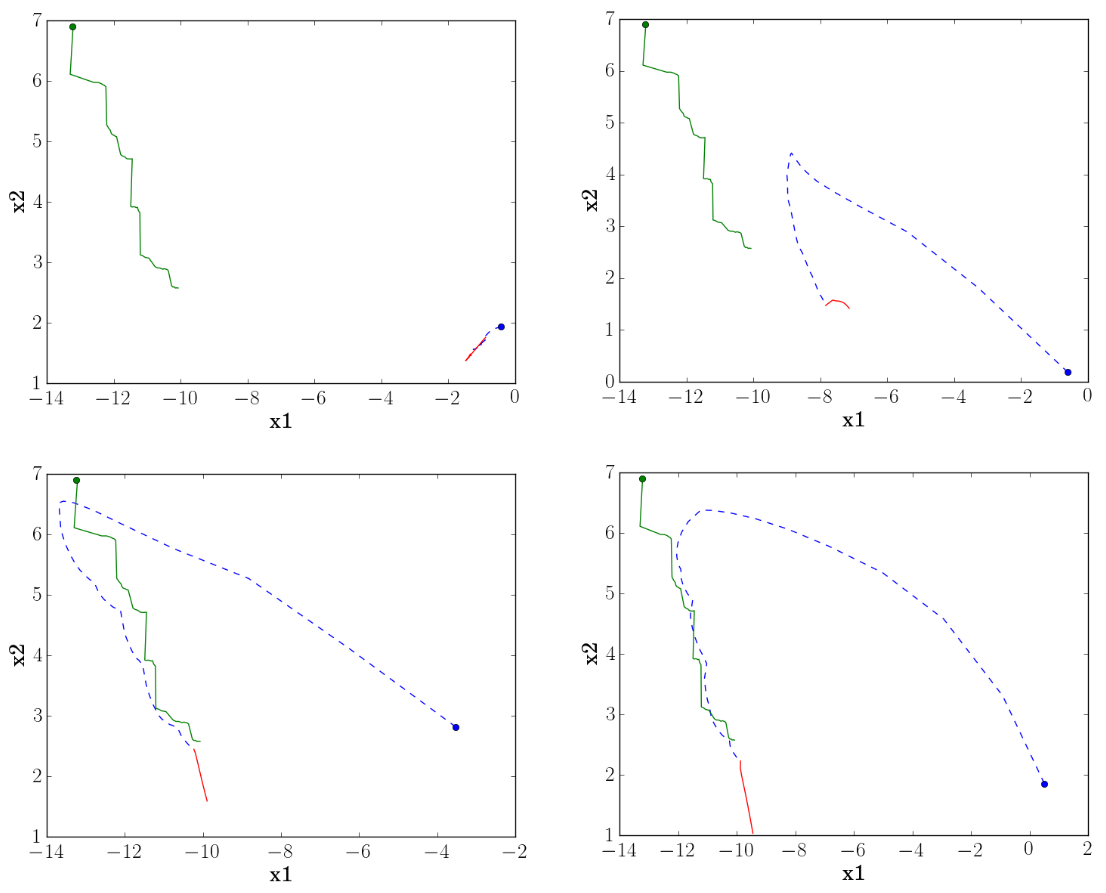
\includegraphics [trim=0 0 0 0, clip, angle=0, width=1.0\columnwidth,
	keepaspectratio]{figures/rnn_real_ped}
	\caption{Search over the number of hidden units: $n_h=1$(top-left), $n_h=4$(top-right), $n_h=32$(bottom-left), $n_h=128$(bottom-right). The plot displays the input trajectory (green) $x_t$ with total trajectory snippet length $T=50$ an its starting point (green-dot). The LSTM predicts the next pedestrian position $y_t$ (blue-dotted) with its starting point (blue-dot), based on the past sequence $x_{0:t}$ and the learned parameters. After the input trajectory (green) is finished, the LSTM tries to predict the future trajectory (red) for $T_p=10$ timesteps. All trajectories are test trajectories and have not been included in the training set.}
	\label{fig:rnn_real_ped}
\end{figure}

\begin{table}[]
\centering
\begin{tabular}{ c| c| c| c| c}
& $n_h=1$ & $n_h=4$ &$n_h=32$ & $n_h=128$\\
\hline
$L_e=0$ & 58.5 & 49.7  & \textbf{6.22} & 2.62      \\
$L_e=1$ & 54.2 & 36.0  & \textbf{0.50} & 0.12      \\
$L_e=2$ & 51.1 & 24.4  & \textbf{0.23} & 0.05      \\
$L_e=3$ & 49.2 & 17.8  & \textbf{0.14} & 0.03      \\
\hline
$e_c$ 			& 25 	& 85 	& 35	& 10 		\\
$L_{e_c}$		&  0.30	& 0.03	& 0.0058& 0.004 	\\
$L_{test, e_c}$	& 0.34	& 0.04	&0.003	& 0.003 	\\     
\end{tabular}
\end{table}

%TODO we have used adam optimizer instead of SGD

\subsection{random stuff}


%TODO oscillating to fit 
In ~\cref{fig:rnn_hidden} (bottom-left), we can see how the error between predicted and true path quickly converges after approximately three timesteps.

\subsubsection{Linear data}

\subsection{Results}



\subsubsection{Hyperparams in bin class}
- Optimize number of hidden units
- batchsize
- learning rate
- maximum epochs


 


- challenge: predict real-valued sequence
- low dimensionality and ease of visualization
- no sophisticated preprocessing or feature-extraction techniques (graves p.18)
	- reduce variation in data (normalize character size, slant, skew,)
- Compare our dataset to handwritten dataset size (graves p.18)
- handwriting has 25 timesteps per character and 700 timesteps per line
- 5000 training, two val of 1500 lines, test 4000 lines (each line 700 tsteps)

\subsection{Network architecture}
- explain $x_t$
	- feeding relative x and y would not respect car position and its influence on pedestrian behavior
- explain $y_t$

\subsection{GRUs}
From: $http://www.jackdermody.net/brightwire/article$
$Sequence_to_Sequence_with_LSTM$

Long Short Term Memory (LSTM) networks are a recurrent neural network that can be used with STS neural networks. They are similar to Gated Recurrent Units (GRU) but have an extra memory state buffer and an extra gate which gives them more parameters and hence a longer training time. While performance with GRU is usually comparable, there are some tasks that each architecture outperforms the other on, so comparing each for a given learning task is usually a good idea.


Number of generated samples: take this from the handwriting paper.
From ~\cref{tab:rnn_hidden}, we have seen how many epochs the model needs to converge. Every epoch repeats training on the same values and thereby increases the probability of overfitting. Therefore, we conclude that we need to train on more data ($N > 5000$), such that the model converges in a low number of epochs and does not overfit.

\subsection{Training}
- Activation unit on output layer
- Optimizer
	- Gradient Descent
		- use momentum?

\subsubsection{Hyperparameters}
- Dropout?!
	- $cell = tf.contrib.rnn.DropoutWrapper(cell, output_keep_prob = args.keep_prob)$

\subsubsection{Regularization}
- Random weight initialization
	- See graves (p.7), weight noise, adaptive weight noise
- use validation set for early stopping
- Gradient clipping?
	- could prove vital for numerical stability
	
\subsection{Results}
- print total loss
- print avg LSE per datapoint


\subsection{Resources}
sunsided $https://github.com/sunsided/tensorflow-lstm-sin$
colah $http://colah.github.io/posts/2015-08-Understanding-LSTMs/$
changhau $https://isaacchanghau.github.io/2017/07/22/LSTM-and-GRU-Formula-Summary/$
hinton 2011 generating text with recurrent neural networks icml 2011